\setAuthor{Andreas Valdmann}
\setRound{piirkonnavoor}
\setYear{2017}
\setNumber{G 3}
\setDifficulty{3}
\setTopic{Dünaamika}

\prob{Pendel}
Nöörist ja koormisest koosnev pendel võngub nii, et amplituudasendis on nööri ja vertikaalsihi vaheline nurk $\alpha=\ang{60}$. Mitu korda erinevad võnkumise käigus suurim ja vähim pinge nööris?

\hint
Koormisele mõjuvad kolm jõudu: niidi pinge, raskuskiirendus ja kesktõmbekiirendus. Lisaks peab resultantjõud olema risti nööriga, sest vastasel juhul peaks koormise kiirenemisel nöör venima või lühenema.

\solu
Olgu pendli pikkus $l$ ja koormise mass $m$. Amplituudiasendis (joonisel vasakul) on pendel paigal ja koormisele mõjuvad raskusjõud $m\vec{g}$ ning nööri pinge $\vec{T}$. Nende jõudude summa $\vec{F}$ on suunatud piki koormise trajektoori ehk on risti nööriga (resultantjõul $\vec{F}$ ei saa olla piki nööri suunatud komponenti, sest vastasel korral peaks koormise kiirendamisel nöör pikenema või lühenema). Täisnurksest kolmnurgast leiame, et amplituudiasendis on pinge nööris $T_1 = mg\cos(\ang{60}) = mg / 2$. Amplituudiasendist eemaldumisel toimub kaks muutust: nurk $\alpha$ väheneb ja koormisele hakkab mõjuma kesktõmbekiirendus, mis on nööri pingega vastassuunaline. Kuna mõlemad muutused suurendavad pinget nööris, siis on pinge vähim just amplituudiasendis.

\begin{center}
	\vspace{-10pt}
	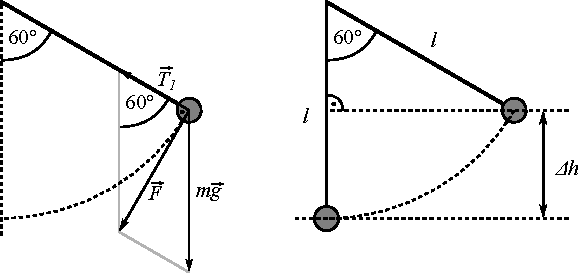
\includegraphics[width=0.65\textwidth]{2017-v2g-03-pendel-joonis.pdf}
	\vspace{-15pt}
\end{center}

Eelnevale argumendile toetudes on pinge nööris suurim pendli tasakaaluasendis: $T_2 = m(g + a)$, kus $a = v^2 / l$ on koormisele mõjuv kesktõmbekiirendus ja $v$ koormise kiirus. Kiiruse $v$ leidmiseks kasutame energia jäävuse seadust, mille kohaselt on koormise potentsiaalse energia muut tasakaaluasendi ja amplituudiasendi vahel võrdne kineetilise energiaga tasakaaluasendis: $mg\Delta h = mv^2 / 2$. Parempoolselt jooniselt näeme, et kõrguste erinevus $\Delta h = l[1-\cos(\ang{60})] = l / 2$. Seega $a = 2g\Delta h / l = g$ ja $T_2 = 2mg$. Niisiis erinevad suurim ja vähim pinge nööris $T_2 / T_1 = 4$ korda.

\probeng{Pendulum}
A pendulum made from a string and a weight is swinging so that at the amplitude position the angle between the string and the vertical direction is $\alpha=\ang{60}$. How many times do the maximal and minimal tensions differ in the string during the swinging?

\hinteng
Three forces apply to the weight: the thread’s tension, gravitational acceleration and the centripetal acceleration. In addition, the resultant force has to be perpendicular to the string because otherwise the string must extend or shorten when the weights accelerates.

\solueng
Let the length of the pendulum be $l$ and the mass of the weight $m$. At the amplitude position (in the left side of the figure) the pendulum is still and gravity force $m\vec{g}$ and tension of the rope $\vec{T}$ are applied to the weight. The sum of the forces $\vec{F}$ is directed along the trajectory of the weight, meaning perpendicularly to the string (the resultant force $\vec{F}$ cannot have a component directed along the string because otherwise the string must shorten or lengthen during the acceleration of the weight). From right triangle we find that at the amplitude position the tension in the string is $T_1 = mg\cos(\ang{60}) = mg / 2$. Two changes take place when withdrawing from the amplitude position: the angle $\alpha$ decreases and the weight is starting to be affected by a centrifugal acceleration that has the opposite direction to the string’s tension. Since both of the changes increase the tension in the string then the smallest tension is indeed in the amplitude position.
\begin{center}
	\vspace{-10pt}
	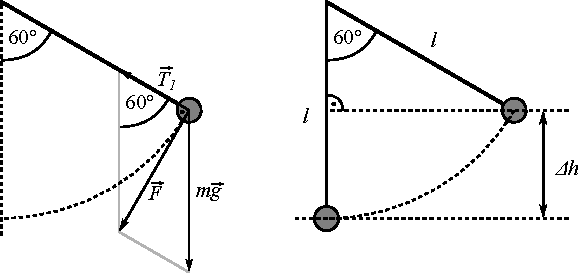
\includegraphics[width=0.65\textwidth]{2017-v2g-03-pendel-joonis}
	\vspace{-15pt}
\end{center}
Relying on the previous argument the tension in the string is biggest in the equilibrium position of the pendulum: $T_2 = m(g + a)$ where $a = v^2 / l$ is the centrifugal force applied to the weight and $v$ the velocity of the weight. To find the velocity $v$ we use the conservation of energy, according to which the potential energy change of the weight between the equilibrium position and amplitude position is equal to the kinetic energy at equilibrium position: $mg\Delta h = mv^2 / 2$. From the figure we see that the difference of heights is $\Delta h = l[1-\cos(\ang{60})] = l / 2$. Thus $a = 2g\Delta h / l = g$ and $T_2 = 2mg$. So the biggest and smallest tension in the rope differ from each other $T_2 / T_1 = 4$ times.
\probend